\section{Results}

Even the most basic area-fitting formulation posed problems for SeDuMi,
which was not able to solve the \gls{sos} problems to a satisfactory optimum
A sample solution is shown in Figure~\ref{fig:sampleSol}, for \gls{sos}
polynomials of order 12.

\begin{figure}
    \begin{subfigure}{0.48\textwidth}
        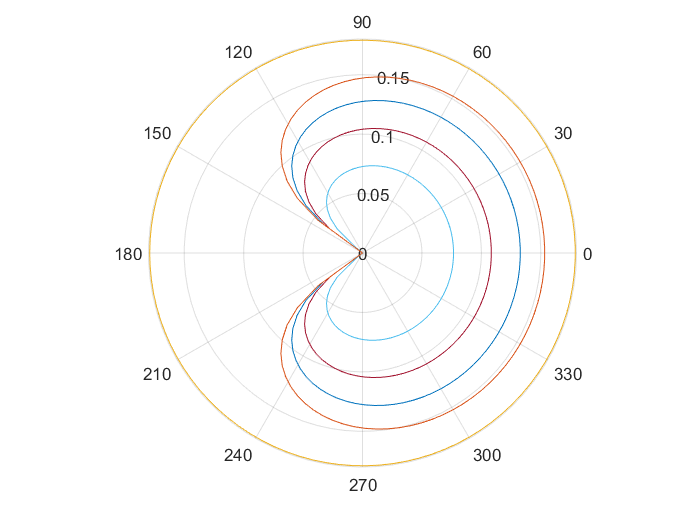
\includegraphics[width = 0.9\linewidth]{figures/sampleSol.png}
    \caption{The shape evolution of the polynomial shows a singulary at the boundaries $-\pi$ and $\pi$.}
        \label{fig:sampleSol}
    \end{subfigure}
    \begin{subfigure}{0.48\textwidth}
        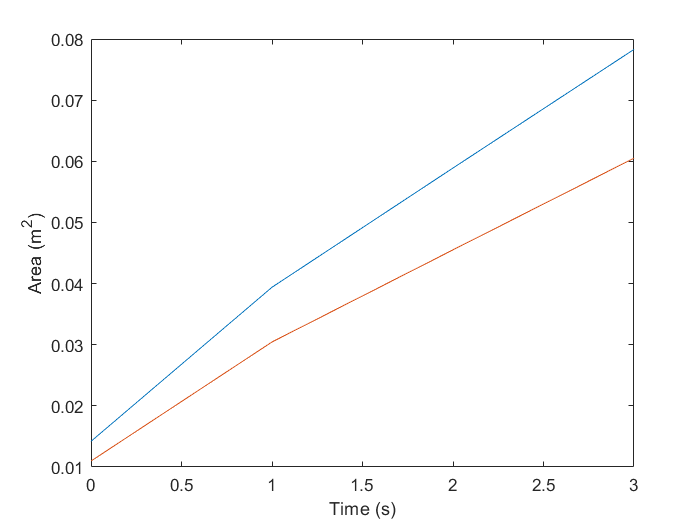
\includegraphics[width = 0.9\linewidth]{figures/sampleA.png}
        \caption{Cross-sectional area evolution of polynomials undershoots the constraints.}
        \label{fig:sampleA}
    \end{subfigure}
    \caption{The simple area-fitting formulation with only L0-continuous boundary condition
    on polynomial fails to return a satisfactory solution.}
    \label{fig:sampleSolandA}
\end{figure}

I believe this has a lot to do with the singularity at the boundary of the domain. This is occurring since the shape is
upper bounded by the outer radius of the rocket, but lower bounded by zero in the domain. I tried a
number of methods to stop a singularity from occurring at the boundary. These included:
\begin{itemize}
    \item Changing the polynomial degrees (odd and even, since my polynomials are
    \gls{sos} only over the interval).
    \item Adding additional regularity conditions (1st and 2nd derivative) at the boundary.
    \item Adding small perturbations at the boundary through inequality constraints.
    \item Making the negative Euclidian distance of the boundary value the objective.
\end{itemize}

None of these attempts worked, although I did notice that the error of the result went down with
increasing degree, so the solver was making some sort of progress.
This is especially odd since it is possible to determine by hand constant
functions $r^2(\theta \in [-\pi, \pi])$ (circles) which satisfy the area constraints,
and yet the \gls{sos} program could not find these.

Frankly, after many hours of tinkering, I am convinced that \gls{sos} programs are not the
right method to tackle this problem. My next step would have been to take
the polynomials, determine their arc lengths, and perturb them with periodic functions (sinusoids)
of appropriate magnitude depending on the distance between the polynomials to ensure that I satisfy
my arc length and area requirements within a specified tolerance.
